

\tableofcontents
\newpage


\section{Introduction}
 
 
 \subsection{Client Side Web Applications}
 \subsection{General remarks}
 \subsection{Structure of this Paper}
\section{Term Definitions}
\section{Analysis of Current Solutions For Developing Client Side Web Applications}
 \subsection{Economical and Technical Advantages of Client Side Web Applications}
 \subsection{Current solutions for Developing Client Side Web Applications}

  At the time of writing (first quarter of 2004), three solutions for developing client side browser based applications exist: JavaScript and Java are two platform independent options for developing the applications, Microsoft's ActiveScripting is an option for applications that only need to run on the MS Windows/Internet Explorer platform.

  \subsubsection{Platform Independent Solutions}
  
   \emph{As stated above, JavaScript and Java are platform independent solution, JavaScript being available on almost any modern web browser and Java as a platform independent programming language. }
   
   \paragraph{JavaScript}
   
    JavaScript/ECMAScript\footnote{The language standardized in the ECMA-262 standard is called ECMAScript by the standard. This name came only up with the standardization of the language and never got used widly, JavaScript is still the more prominent name and will be used} is the common name for the scripting language defined in ECMA standard 262. It was originally developed
% as JavaScript 
by Brendan Eich at Netscape. The purpose of JavaScript was to give web developers the posibility create interactive HTML documents; JavaScript is integrated with Netscape's Navigator web browser since version 2.0. An alternative implementation of a JavaScript interpreter was developed by Microsoft. This interpreter however was not bound directly to Microsoft's Internet Explorer web browser but integrated into it using ActiveX/OLE/COM(?). The Microsoft JavaScript interpreter however is not fully compatible to Netscape's interpreter; the Microsoft derivative of JavaScript is called \emph{JScript}. The JScript interpreter is bundled with the Internet Explorer starting with its 3.0 release. Microsoft's approch to client side browser scripting however is not limited to JScript, section \ref{sec:activescripting} gives more information on this.

The development of the standard for the JavaScript language, standardized as ECMAScript, started in November 1996; the standard was adopted first in June 1997. It was also accepted as ISO/IEC standard 16262 in April 1998. As of February 2004, the standard is in its third edition and availabe from \cite{ECMA-262}, which correspondes to JavaScript 1.5.

%ECMA262: http://www.ecma-international.org/publications/standards/Ecma-262.htm
%	+ pdf document

JavaScript is now available -- to different extents -- in all relevant web browsers; additionally, stand-alone JavaScript interpreters exist that allow the use of JavaScript as a standalone script language not limited to in-browser use. One of the most prominent of these interpreters is the Rhino JavaScript interpreter maintained by and available from The Mozilla Organisation.

%mozilla.org, mozilla.org/rhino, availablity of JS in browsers?

For use as client side scripting language in web applications, JavaScript has some important disadvantages:

\begin{description}
	\item[Limited Possibilites] The possibilites provided by standard conform JavaScript are very limited. Java\-Script only allows interaction with its parent document\footnote{The document that embedds or references the script.}, not with any system or network ressources. Tasks that require for example file system, database or network access are not possible with standard conform JavaScript.\footnote{These limitations do not apply to Microsoft's JScript, cf. section \ref{sec:activescripting}.} 
	\item[Missing Standard Conformance] Another problem with Java\-Script based solutions is that although Java\-Script is standardized, different browsers interpret the same JavaScript code differently and any non-trivial application based on JavaScript has to be customized to the browser platform it will be used on. For an application that has to work on different platforms, for example Opera and Internet Explorer, some parts have to be coded for each browser separatly along with code deciding at run time which browser it runs on and which code is the one that must be used. A consequence of this is that JavaScript applications get overly complex and \emph{expensive} when the resulting application shall be availble on multiple browsers.
\end{description}

However, JavaScript also has some important advantages:
\begin{description}
	
	\item [Easy to Learn] JavaScript is a loose typed language, the syntax is a mix of elements from C and Java and a lot of simple examples and tutorials is available for free on the web.\footnote{E.g. at \cite{W3SchJS}} Additionally, nothing but a web browser is necessary to start programming with JavaScript.
	
	\item [Wide User Base] JavaScript is integrated in all relevant browsers and thus provides a wide user base that can use JavaScript applications 'out of the box'. As JavaScript is always available when a web browser is installed,, no costs of maintaining or installing JavaScript accumulate.
	
	\item [Secure] As JavaScript implementations conforming to the standard do not allow operations outside of their designated are -- their parent document -- potentially hazardous actions like reading content from other browser windows or accessing the local file system are theoretically not possible.\footnote{This does not to the JScript security model, cf. section \ref{sec:activescripting}.}
	
\end{description}
    
   \paragraph{Pure Java}
   
    Java is an object oriented programming language developed by Sun and available since 1995. Java, from the beginning of its development, was designed to be a platform independent programming language: The concept of Java consists of a 'two-step' approach in compiling and running Java programs: The Java source code is compiled into a architecture neutral bytecode; upon running, that bytecode is interpretet by the Java virtual machine that must be available on the computer running Java application.

One of the most important reasons why Java was created platform independant was the intention to use Java as a programming language in heterogenous environments, especially the internet, where platform independence make it possible to write applications once and run them on any desired platform.

%JAVA PLUGIN

Another feature of Java is that it allows the creation of applications that can be embedded in HTML documents: Java applets. These applets reside in and control a designated area of the HTML document. As Java, in contrast to JavaScript, is a full featured language, these applets could potentially be dangerous. To allow the use of Java applets without compelling users to check the security of the applets, Java created a secure environment, the sandbox, for Java applets that allows only safe operations; in order to allow potentially harmful tasks like filesystem access, this sandbox can be left when the user explicitly allows this. The security model of the Java sandbox is fine-grained, the user can specify exactly which applet should have which permission (which files may be accessed, which hosts contacted over the internet, ...). 

The Java Standard Edition comes with hugh class library that provides classes for most standard tasks like reading files from local and remote locations, database access or TCP/IP connections. All of this functionality is available in Java applets.


Current versions of the Java plugin also allow applets access to elements of browser documents. 

However, compared with JavaScript, interaction with document elements is much more complicated. 




In a nutshell, the disadvantages of Java are:

\begin{itemize}
	\item It is much harder to learn than most scripting languages.
	\item Interaction between Java and web browsers is more complicated than it is with 'browser native' languages.
	\item Java code must be compiled, it can not be changed at runtime.
	
\end{itemize}

Advantages of Java are:

\begin{itemize}
	\item Java is a truely platform independent programming language available on all major operating system and hardware platforms.
	\item Java comes with a huge class library.
	\item Program execution is much faster than it is with scripting languages.
	\item Java code distributed over the internet runs in a safe environment.
\end{itemize}
    
  \subsubsection{A Proprietary Solution: Microsoft ActiveScripting}
  \label{sec:activescripting}
  
\section{BWS}
 \subsection{Technical Overview}
 \subsection{Base Technologies}
  \subsubsection{DOM}
  
    The DOM 
\begin{quotation}
	is a platform- and language-neutral interface that will allow programs and scripts to dynamically access and update the content, structure and style of documents.\footnote{w3dom,whatis}
\end{quotation}
%ref http://www.w3.org/DOM/#what

It is standardized by the W3C DOM working group which accepts submissions from member companies and tries to implement their wishes in a interoperable and scripting-language neutral solutions.

   
   \paragraph{DOM Basics}
   
    
DOM objects are hierarchically organized into a DOM tree with the topnode of a XML document as the root object of the DOM tree. Every part of a XML document correspondes to a DOM object: The following code snippet of a XML document is mapped to the tree shown in figure \ref{fig:simpleDomTree}.

\begin{verbatim}
<html>
 <head>
  <title>DocumentTitle</title>
 </head>
 <body>
  <h1 id="aHeading">Heading</h1>
  <br />
  <p id="aParagraph" style="fontFamily:sans-serif;">Content</p>
 </body>
</html>
\end{verbatim}

\begin{figure}[htbp]
	\centering
		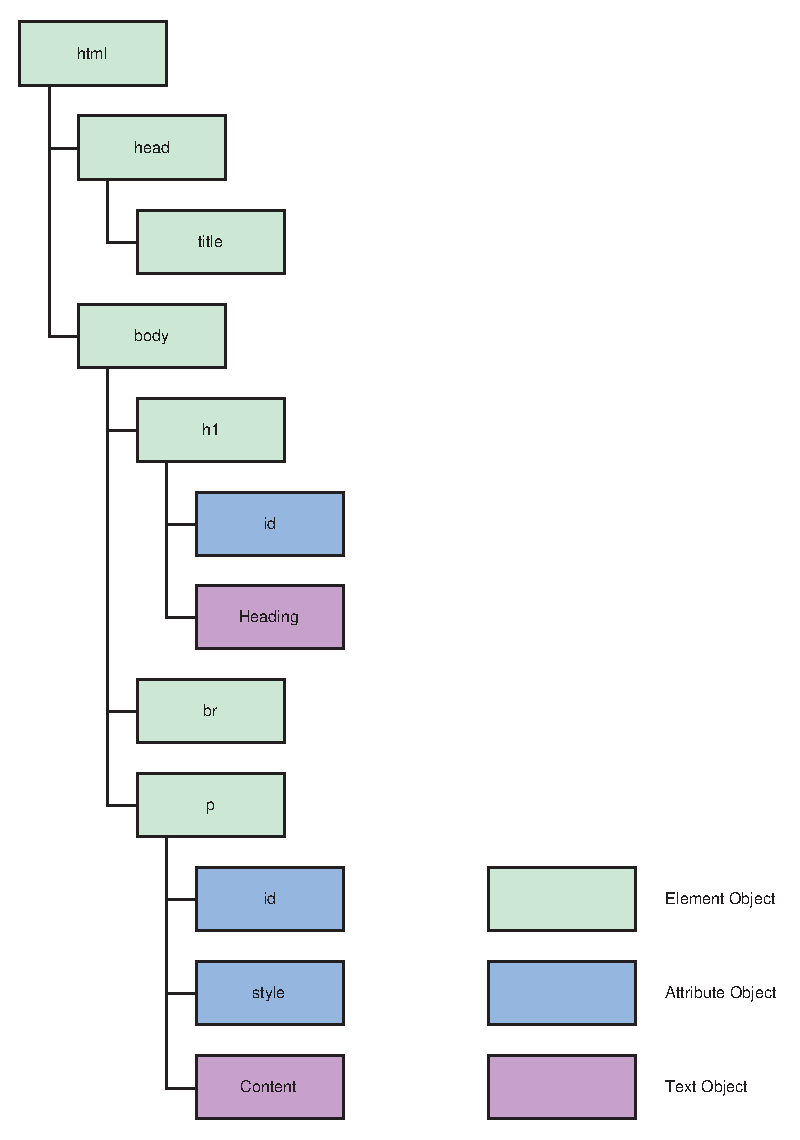
\includegraphics[scale=0.5]{simpleDomTree}
	\caption{SDT}
	\label{fig:simpleDomTree}
\end{figure}

The figure showes three types of DOM 'classes': 

\begin{enumerate}
	\item Element objects, these correspond to XML tags and are characterized by there type, e.g. a \texttt{h1} or a \texttt{title}.
	\item Attribute objects, these correspond to XML attributes and are name-value pairs, e.g. the paragraphs \texttt{style} value is \texttt{Heading}.
	\item Text objects, the part of the document between the tags that is the (unstructured) content of document.
	
\end{enumerate}

Properties and methods available for these DOM classes are also definined in the DOM standard; DOM for example defines that each element node may have an attribute \texttt{id} and that every element node supports the method \texttt{appendChild} that expects another node as argument and attaches this node to the node the method is invoked on.


    
   \paragraph{DOM in Java: dom4j}
    
    In order to work with these objects, it is necessary that they are available in the programming language used; in this case this is Java.

One of the solutions available for mapping DOM objects to Java objects is the open-source solution dom4j. This framework enables the parsing of XML documents to Java objects, the navigation and modification of parts of the represented XML document as well as the creation of a XML document from the Java objects.

dom4j provides two ways of accessing the Java objects corresponding to a specific DOM element: The first one is to walk the DOM tree hierarchically that is, iterate over all elements of the lowest layer, check if one of the elements of this layer match the desired criteria, then select all of the elements of the next lower layer and do the same for all layers until the desired element is reached. 

For example if in figure \ref{fig:simpleDomTree} the heading's content is wanted, the procedurce would have to look like this:

\begin{enumerate}
\item Select all child elements of the \texttt{html} node.
\item Check if the elements type is \texttt{body}.
\item If it is \texttt{body}, select all child elements of this element.
\item Iterate over these elements and check if they are \texttt{h1} elements.
\item If a element is a \texttt{h1}, select its content.
\end{enumerate}

As this method is very laborious and time consuming, especially for complex and large XML documents, dom4j provides another way of selecting the desired elements: the XML Path Language (XPath).

    
   \paragraph{Selecting DOM Elements: XPath}
   
    XPath, standarized by the W3C is a XML element query language: It allowes to specify certain criteria that are then used to select all elements of a XML document that match these criteria. The easiest way is specifying the path to an element, to address the \texttt{h1} element in figure \ref{fig:simpleDomTree}, the apropriate XPath expression would be \verb|/html/body/h1|, that is, the root element (\verb-/-) and all relevant children types separated by (forward) slashes.

For selecting the \texttt{h1} content, the procedure would be this:

\begin{enumerate}
	\item Select the \texttt{h1} element with XPath using \verb|/html/body/h1|.
	\item Get this element's content.
\end{enumerate}

However, this way of selecting elements is still based on the full path of the elements within the DOM tree and does not allow accessing elements only by type (without specifying a full path). For this purpose, XPath provides the posibility to select elements independent from their path. XPath expressions using this method start with a double slash (\verb|//|) instead of the single root slash. The expression for selecting all \texttt{h1} elements in a document therefore would be \verb|//h1|.

This would allow to use the following procedure for selecting the \texttt{h1} content:

\begin{enumerate}
	\item Select all \texttt{h1} elements with XPath using \verb|//h1|.
	\item Get all selected elements' content.
\end{enumerate}

The difference between the two examples using XPath above is that the second example would return any \texttt{h1} element within the document independant of its position (i.e. it would also return a \texttt{h1} lying under the \texttt{p} element in the given document whereas the first expression would only reply \texttt{h1} elements that are exacly in the third layer of the document and have \texttt{html/body} as parents.
   
   \paragraph{Modifiying the DOM in Java with dom4j}
   
    The first step in modifying an existing\footnote{dom4j also provides the possibility to build DOM trees/XML documents form scratch. As this possibility is not used in BWS, it is not \emph{detailed} in this paper.}  DOM in Java is parsing the DOM underlying XML document and building the DOM tree in Java. dom4j uses the Simple API for XML (SAX)\footnote{SAX is available from \cite{SaxHP}} for this purpose.

%saxhp=www.saxproject.org

Reading the XML document is done by using a \texttt{org.dom4j.io.SAXReader} objects \texttt{read()} method on the source of the XML document; the source may be a \texttt{String}, an \texttt{URL}, a \texttt{InputStream}, a \texttt{Reader} or a \texttt{org.sax.InputSource}. This method returns a DOM tree as an \texttt{org.dom4j.Document}.

The root element of the parsed document can then be obtained using the \texttt{getRootElement()} method on the document returned from the \texttt{SAXReader}. Elements in dom4j are objects of the class \texttt{org.dom4j.Element}.

To allow access to child elements of the current element, each \texttt{Element} provides a standard Java \texttt{Iterator} that allows iteration over all child objects. Figure \ref{fig:AMinimalDom4jExample} shows a minimal dom4j example that provides two methods: \texttt{parseDocFromURL()} to read an XML document from an URL and \texttt{printRootChildren()} to print the element types of all direct child nodes of the root element of the document read with the \texttt{parseDocFromURL()} method.

\begin{figure}[htb]
  \begin{verbatim}
import java.util.Iterator;
import java.net.URL;

import org.dom4j.*;
import org.dom4j.io.SAXReader;

public class Dom4jExample {
  private Document dom4jDocument;
  
  /* SAXReader.read() throws a DocumentException when problems reading
   * or parsing an XML document occur, for example if the document is
   * not available at the specified place or if it is not well-formed.
   */
  public void parseDocFromURL(URL anURL) throws DocumentException {
    SAXReader xmlReader = new SAXReader();
    this.dom4jDocument = xmlReader.read(anURL);
  }
  
  public void printRootChildren() {
    Element documentRoot = this.dom4jDocument.getRootElement();
    
    Iterator elementIterator = documentRoot.elementIterator();
    
    // iterate over all children
    while(elementIterator.hasNext()) {
      Element currentElement = (Element)elementIterator.next();
      System.out.println(currentElement.getName());
    }
  }
}
  \end{verbatim}
	
	\caption{A minimal dom4j example}
	\label{fig:AMinimalDom4jExample}
\end{figure}
    
  \subsubsection{LiveConnect and the Sun Java Plugin}
  \subsubsection{BSF}
  \subsubsection{Relations Between the Base Technolgies}
 \subsection{Classes and Their Relations}
 \subsection{BWS in Action}
  \subsubsection{The Details of Document Rewriting}
   \paragraph{The BWSDocument class}
   \paragraph{Using BWSDocument}
    \subparagraph{Server-side}
    \subparagraph{Client-side}
  \subsection{The Details of Application Execution}
   \subsubsection{The BWSApplet}
   \subsubsection{The ScriptString Class}
   \subsubsection{The JSNode Class}
\section{Discussion}

\section{Using BWS}

 \subsection{An Example of BWS in Action}
 \subsection{Installing BWS}
 \subsection{Creating BWS Applications}
 
  \subsubsection{XHTML Documents as Starting Point for BWS Applications}

  The starting point of a BWS compliant document is a standard well-formed HTML document, that is, it must fullfil the following requirements\footnote{There are some additional requirements that do not apply to BWS documents, see \cite{references}, the exact requirements of well-formedness for XML documents is \cite{w3reference}:

\begin{itemize}

\item For every start tag, there must be a closing tag, i.e. for every \ttfamily{<li>} tag there must be a \ttfamily{</li>} tag; an exception to this rule is allowed for tags that have no content, e.g. \ttfamily{<br>}, these tags must be given in the combined notation \ttfamily{<br/>}. As some browsers do not accept the later variant, it is recommended to use explicit start and end tags and, in cases where this is not possible, seperate the closing slash by a space from the tag itself, e.g. \ttfamily{<br />}. This notation should work with any BWS supporting browser.

\item Elements can have subelements, they must use strict nesting, 'overlapping' tags, for example \ttfamily{<h1>Text<center>Centered</h1>also centered</center>}, are not allowed.

\item Tags and attributes are case-sensitve, for example \ttfamily{<h1>} and \ttfamily{</H1>} are not matching.

\item Attributes must have exactly one value, empty attributes that are allowed in standard HTML, e.g. the \ttfamily{mayscript} attribute of objects must be given as \ttfamily{<object mayscript="true" />}, not only \ttfamily{<object mayscript>}, all attributes must be enclosed in quotes.

\item The document must have exactly one root element, i.e. a construction \ttfamily{<html><!-- htmlcode --></html><somethingElse></somethingElse>} is not allowed. 

%example in figure? multiline?

\end{itemize}

Any document conforming to these requirements can be used as a BWS document and extended with BWS scripts; generally, an XHTML compliant document will work. For an example an incorrect document as well as a corrected version of this document (changes are emphasized), see figure \ref{fig:xhtmlDocumentExample}. 

\begin{figure}
\label{fig:xhtmlDocumentExample}

%preformated

<html>
<head>
<Title>An incorrect document</title>
</head>

<body>
<h1>This is a heading<H1>
<div>This is <em>the first part</div></em>
<p>A new paragraph.
<p>And another one.<br>
The last one ended with a linebreak.
</body>

</html>

The incorrect document.


<html>
<head>
<_t_itle>An incorrect document</title>
</head>

<body>
<h1>This is a heading<_H_1>
<div style=_"_fontFamily:Verdana_"_>This is <em>the first part_</em></div>_
<p>A new paragraph._</p>_
<p>And another one._</p><br >_
The last one ended with a linebreak.
</body>

</html>

A corrected version.


\end{figure}

%references http://www.intelligenteai.com/XMLRepository/well_formed_xml_document.htm
%			http://www.w3.org/TR/2000/REC-xml-20001006#sec-well-formed

  \subsubsection{Embedding And Referencing Scripts}

 Once you've got a BWS compliant document as described above, you can embed you scripts. This step consists of two parts: 

\begin{enumerate}

\item Embed or reference the scripts in the document.

\item Attach script calls to the events you want to catch.

\end{enumerate}

Both steps are done almost exactly like they would be done using JavaScript scripts.

%paragraph or only highlighting?
\paragraph{Embedding and referencing scripts}

For every script you want to use, create a \texttt{<script>} tag. This script tag must have at least two attributes:

\begin{enumerate}

\item The \texttt{type} attribute that specifies that this script is a script that shall be interpreted using BWS and the programming language the script is written in; this attribute is given as \texttt{bws/scriptengine}, for example it is \texttt{bws/netrexx} for the NetRexx interpreter or \texttt{bws/javascript} for the Rhino JavaScript interpreter.

\item The \texttt{id} attribute unter which this script is referenced in script calls. This id, as well as any other id used in the document, must be unique, it may consist of only alphanumeric characters (A-Z, a-z, 0-9), dashes (-), underscores (\_), dots (.) and colons (:).

\end{enumerate}

If only these two attributes are specified, the script code must be embedded within the script element (see figure /ref{fig:scriptEmbedding}); if the script code shall not be contained within the document, it is also possible to reference scripts contained in extra files. To do this, the optional source attribute \texttt{src} can be specified. This attribute has to be in the form of an absolute\footnote{(e.g. \texttt{http://location/filename})} or a relative\footnote{Relative to the URL of the document, e.g. if the document is available from http://www.mydomain.com/aDocument.html and the script file is available from \texttt{http://www.mydomain.com/scripts/aScript.bws}, it can also be referenced as \texttt{scripts/aScript.bws}} URL; using this method, the script file is loaded only on execution. If the \texttt{src} attribute is specified, the code under the script element is not inspected.

%caching when referencing is used

Other tags may be specified too, but are not used by BWS (they may be used by the browser).

\begin{figure}[htb]
	\label{fig:EmbeddingAndReferencingScripts}
	Embedding scripts
	\ttfamily 
	\begin{verbatim*}
	<html>
	...
	<script type="bws/netrexx" id="aRexxScript">
	-- some netrexx code
	</script>
	...
	</html>
	\end{verbatim*}
	\rmfamily
	
	Referencing scripts
	
	\ttfamily
	\begin{verbatim*}
	<html>
	...
	<script type="bws/netrexx" id="aRexxScript" src="./rexxscript.bws" />
	...
	</html>
	\end{verbatim*}
	
	\rmfamily
	\caption{Embedding and Referencing Scripts}

\end{figure}

\paragraph{Attaching script calls to events}

After all necessary scripts are embedded or referenced in the document, script calls can be attached to events, i.e. scripts can be triggered by DOM events, for example by clicking a part of text. For an overview which events are available, see \cite{ReferenceDOMEvents}.
%notcitedyet

Scripts can be attached to any event of any element using the syntax \texttt{bws:scriptId} as the eventhandler. For example if you have a script with the id \texttt{myOnClickScript} you would like to call when the body of your document is clicked, the body tag must be:

\ttfamily

\begin{verbatim*}
<html>
...
<body onclick="bws:myOnClickScript">
...
</body>
</html>
\end{verbatim*}

%references in this document part
%attributes for scripts: http://selfhtml.teamone.de/html/referenz/attribute.htm#script
%universal attributes: http://selfhtml.teamone.de/html/referenz/attribute.htm#universalattribute

  \subsubsection{Accessing And Modifiying DOM Elements}

  %\include{accessingDOM.tex}

 \subsection{Advanced Possibilities of BWS}
  \subsubsection{An Extension to the Given Example}
  \subsubsection{Calling Scripts from Other Scripts}
  \subsubsection{Passing Parameters and Returning Values from BWS Scripts}
 \subsection{Code Comparison: BWS and JavaScript}
\section{Wrap-Up and Outlook}